\subsection{Giao diện người dùng}
\label{chap:ui}

Pipeline dữ liệu chỉ có giá trị khi kết quả của nó đến được tay người dùng. Mục này trình bày ứng dụng web phục vụ năm nhóm người dùng: người học, giảng viên, cố vấn học tập, quản trị viên tổ chức và đội vận hành nền tảng dữ liệu.

\subsubsection{Quy trình thiết kế}

Nhóm dùng mockup HTML để thử bố cục theo vai trò, rồi hiện thực giao diện React và TypeScript trong \code{apps/web}. Instructor đọc kết quả đánh giá có phiên bản, Advisor đọc đặc trưng rủi ro và vòng đời cảnh báo, còn Admin đọc báo cáo theo tổ chức. Các ảnh dưới đây lấy từ bản giao diện đã triển khai. Kịch bản Replay có nhãn dữ liệu mô phỏng.

\subsubsection{Hệ thống thiết kế}

\begin{itemize}
  \item \textbf{Token thiết kế} cho màu, khoảng cách, bo góc và bóng đổ, có bộ giá trị riêng cho chế độ sáng và tối. Người dùng chuyển chế độ bằng một công tắc; mặc định là chế độ sáng.
  \item \textbf{Bảng màu biểu đồ đã kiểm định}: màu phân loại theo thứ tự cố định và một dải màu xanh đơn sắc cho độ lớn (heatmap), đã kiểm tra khả năng phân biệt với người mù màu. Màu trạng thái (tốt, cảnh báo, nghiêm trọng, nguy hiểm) chỉ dùng cho trạng thái và luôn đi kèm biểu tượng và nhãn chữ, không bao giờ chỉ dựa vào màu.
  \item \textbf{Khả năng tiếp cận}: mọi biểu đồ có tooltip khi rê chuột và một bảng dữ liệu ``Xem dạng bảng'' thay thế; các nút có nhãn cho trình đọc màn hình; bố cục co giãn tới màn hình điện thoại mà không phải cuộn ngang.
  \item \textbf{Nhãn yêu cầu}: mỗi trang và mỗi khối được gắn nhãn BR tương ứng (có thể tắt). Nhãn này giúp truy vết từ giao diện về yêu cầu khi trình bày.
\end{itemize}

\subsubsection{Kiến trúc frontend}

Ứng dụng tổ chức theo \emph{không gian làm việc} (workspace), mỗi nhóm người dùng một workspace, chọn ở thanh bên (Bảng~\ref{tab:routes}). Thanh trên cùng có chỉ báo sự kiện trực tiếp (Server-Sent Events), thông báo của người học và trạng thái đăng nhập.

{\small
\begin{longtable}{@{}L{2.4cm}L{4.4cm}L{6.4cm}L{1.4cm}@{}}
\caption{Workspace, đường dẫn và trang}\label{tab:routes}\\
\toprule
\textbf{Workspace} & \textbf{Đường dẫn} & \textbf{Nội dung} & \textbf{BR} \\
\midrule
\endfirsthead
\toprule
\textbf{Workspace} & \textbf{Đường dẫn} & \textbf{Nội dung} & \textbf{BR} \\
\midrule
\endhead
Learner & \code{/learner} & Khoá học, gợi ý, phản hồi gần đây, thông báo & 1, 2 \\
Learner & \code{/learner/code-lab} & Trình soạn mã, phản hồi từng test, các lần nộp & 3 \\
Instructor & \code{/instructor/assessments} & Câu hỏi và chi tiết test case & 4 \\
Instructor & \code{/instructor/videos} & Heatmap theo phiên bản, lớp phủ hôm nay, thời điểm cần xem lại & 7 \\
Instructor & \code{/instructor/engagement} & Trung bình khoá học, học viên đang giảm & 8 \\
Instructor & \code{/instructor/content} & Xuất bản phiên bản, theo dõi đồng bộ, xem trước tìm kiếm & 8 \\
Advisor & \code{/advisor} & Hàng đợi rủi ro, phân rã điểm, lịch sử, cảnh báo & 5 \\
Org admin & \code{/admin} & Tiến độ tổ chức có ẩn nhóm nhỏ, xuất CSV & 6 \\
Data platform & \code{/pipeline} & Bộ đếm luồng, thông lượng, topic, DLQ, silver & -- \\
\bottomrule
\end{longtable}}

\subsubsection{Xác thực và phạm vi dữ liệu}

Trong Classroom, người học đăng nhập bằng tài khoản học viên và đọc bài nộp theo quyền sở hữu. Instructor, Advisor và Organisation Admin dùng tài khoản cấp sẵn trong \code{EDU_STAFF_ACCOUNTS} ở Classroom, Persistent và Replay. Lệnh cấp tài khoản nhận mật khẩu từ lời nhắc ẩn và xuất hash Argon2id~\cite{argon2cffi}. Máy chủ đặt cookie HttpOnly, SameSite=Strict và bật Secure trên HTTPS. Mỗi vai trò có một phiên tám giờ trên trình duyệt, độc lập với vai trò khác và Student. Đăng xuất thu hồi phiên tương ứng. Khởi động lại API kết thúc các phiên staff trong tiến trình.

Ứng dụng gửi \code{X-Staff-Role} để máy chủ chọn cookie phiên. Máy chủ kiểm tra vai trò, phạm vi khóa học hoặc tổ chức và cùng origin đối với thao tác ghi bằng cookie. Script có thể dùng Bearer token khai báo trong \code{EDU_BR45_AUTH}. Khi Trino chưa sẵn sàng, Admin vẫn đăng nhập và trang báo cáo hiển thị lỗi tải dữ liệu.

\begin{figure}[htbp]
\centering
\begin{subfigure}{0.48\textwidth}
  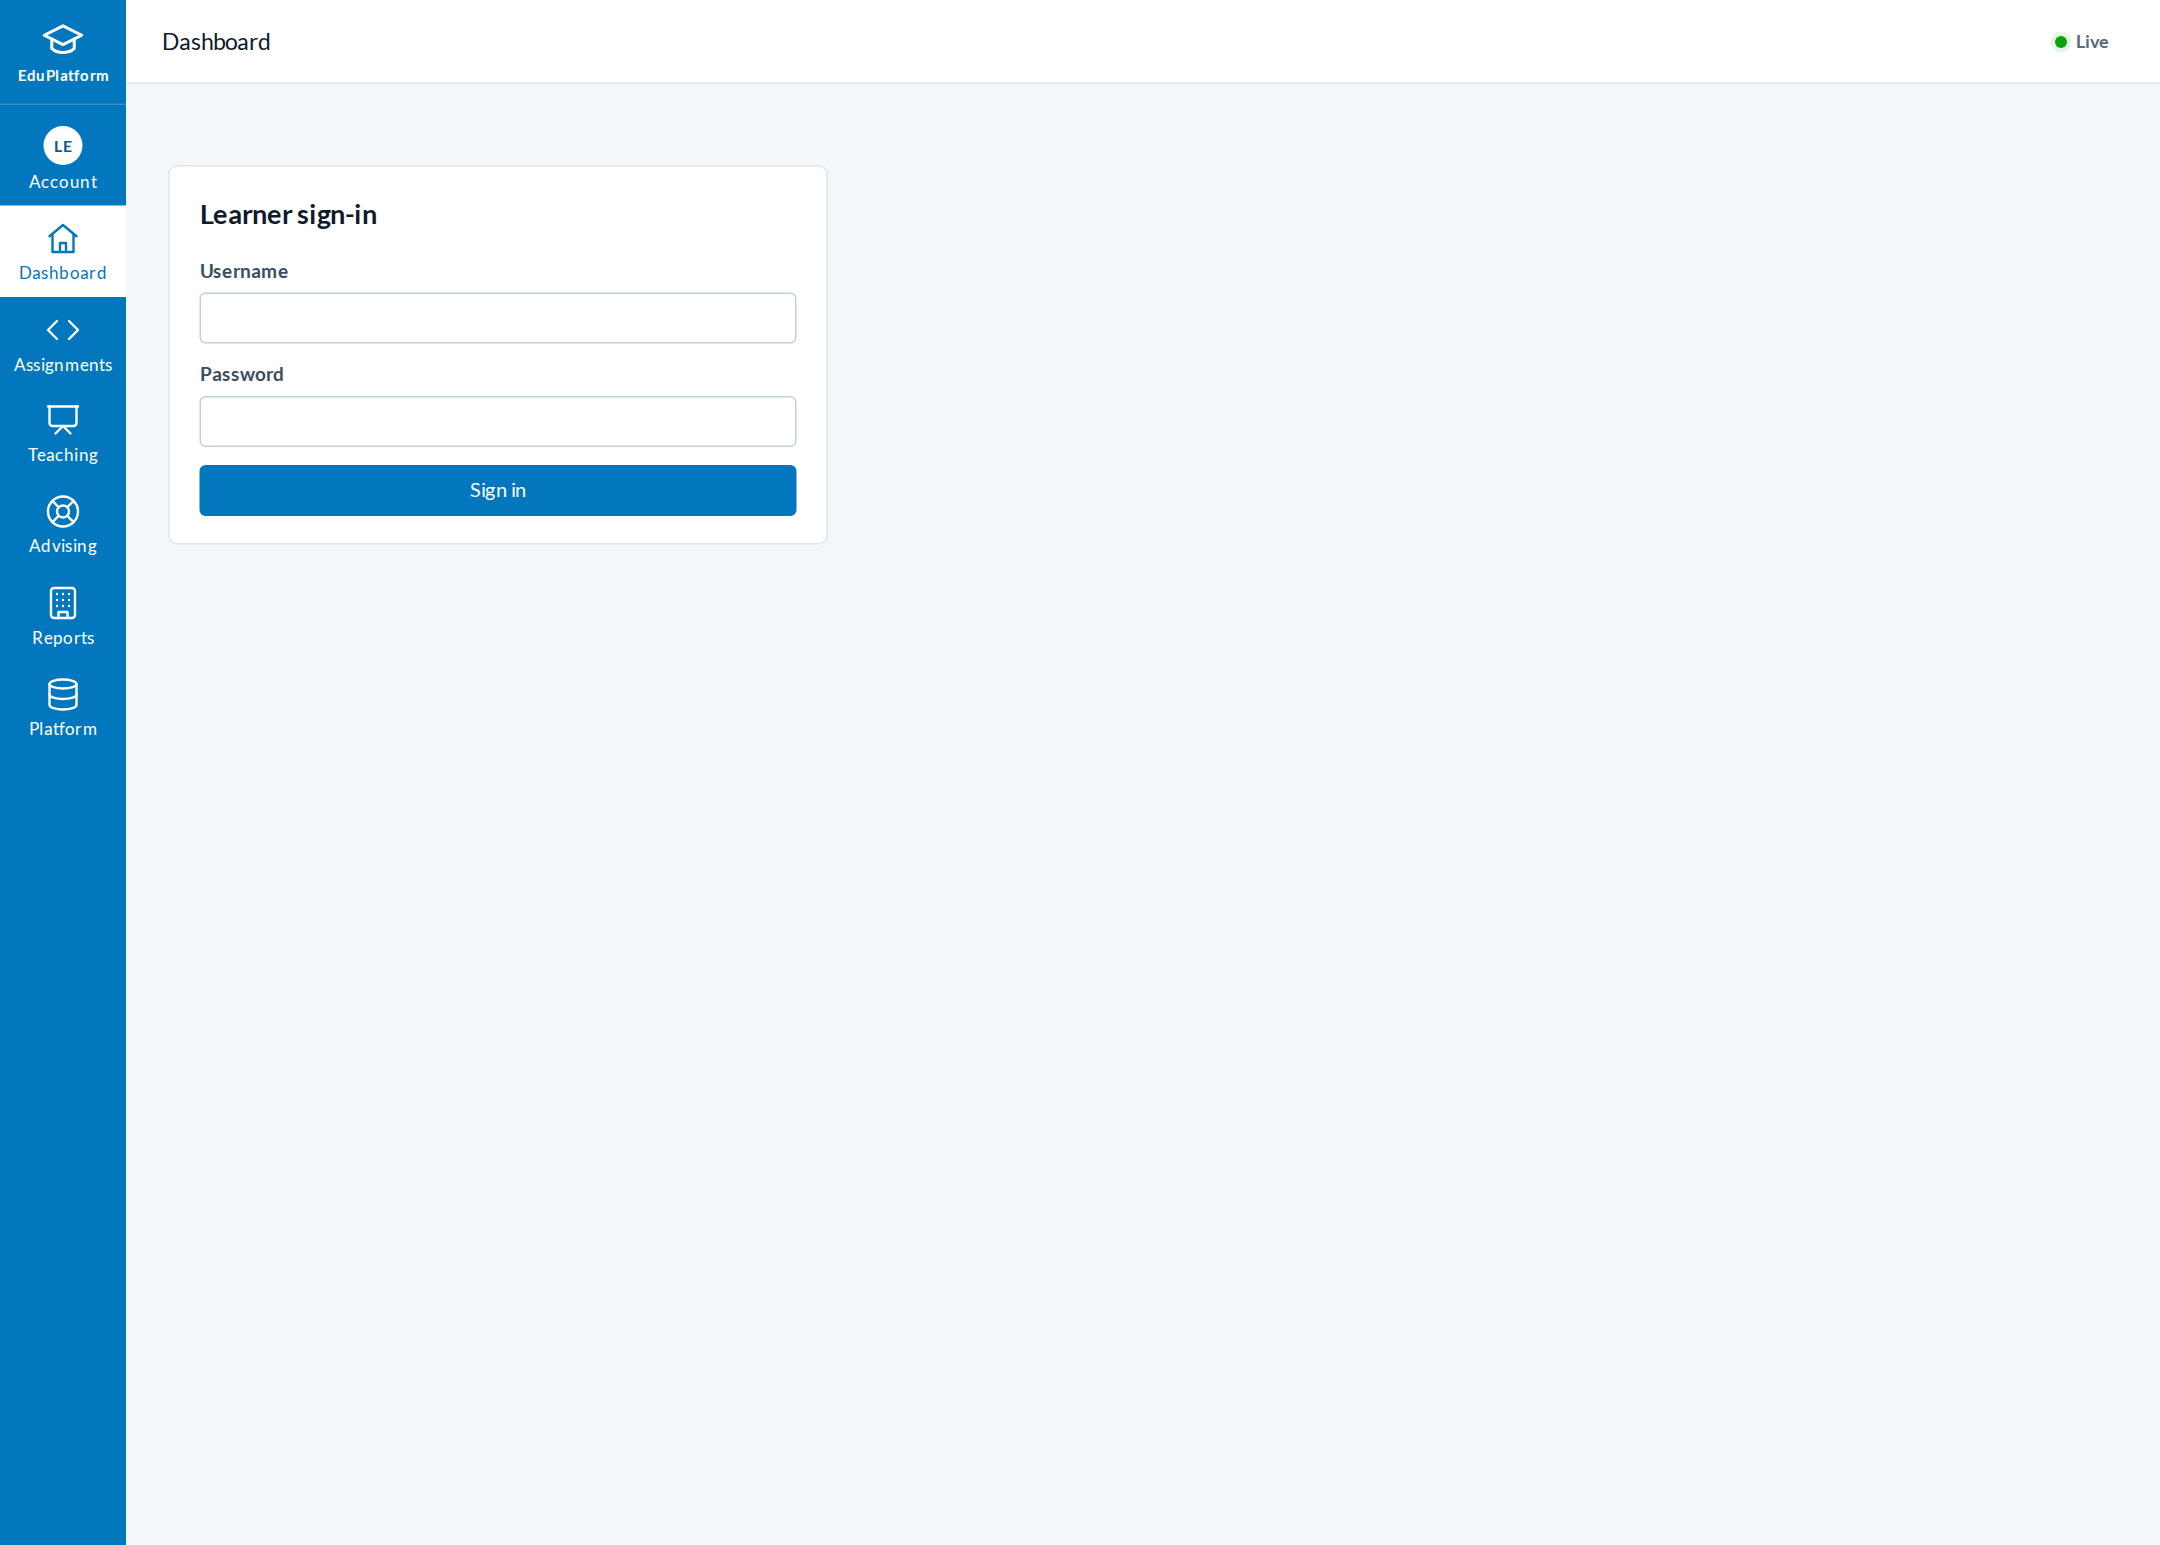
\includegraphics[width=\linewidth,trim=0 535bp 820bp 0,clip]{figures/current/auth-student.png}
  \caption{Student, Classroom}
\end{subfigure}\hfill
\begin{subfigure}{0.48\textwidth}
  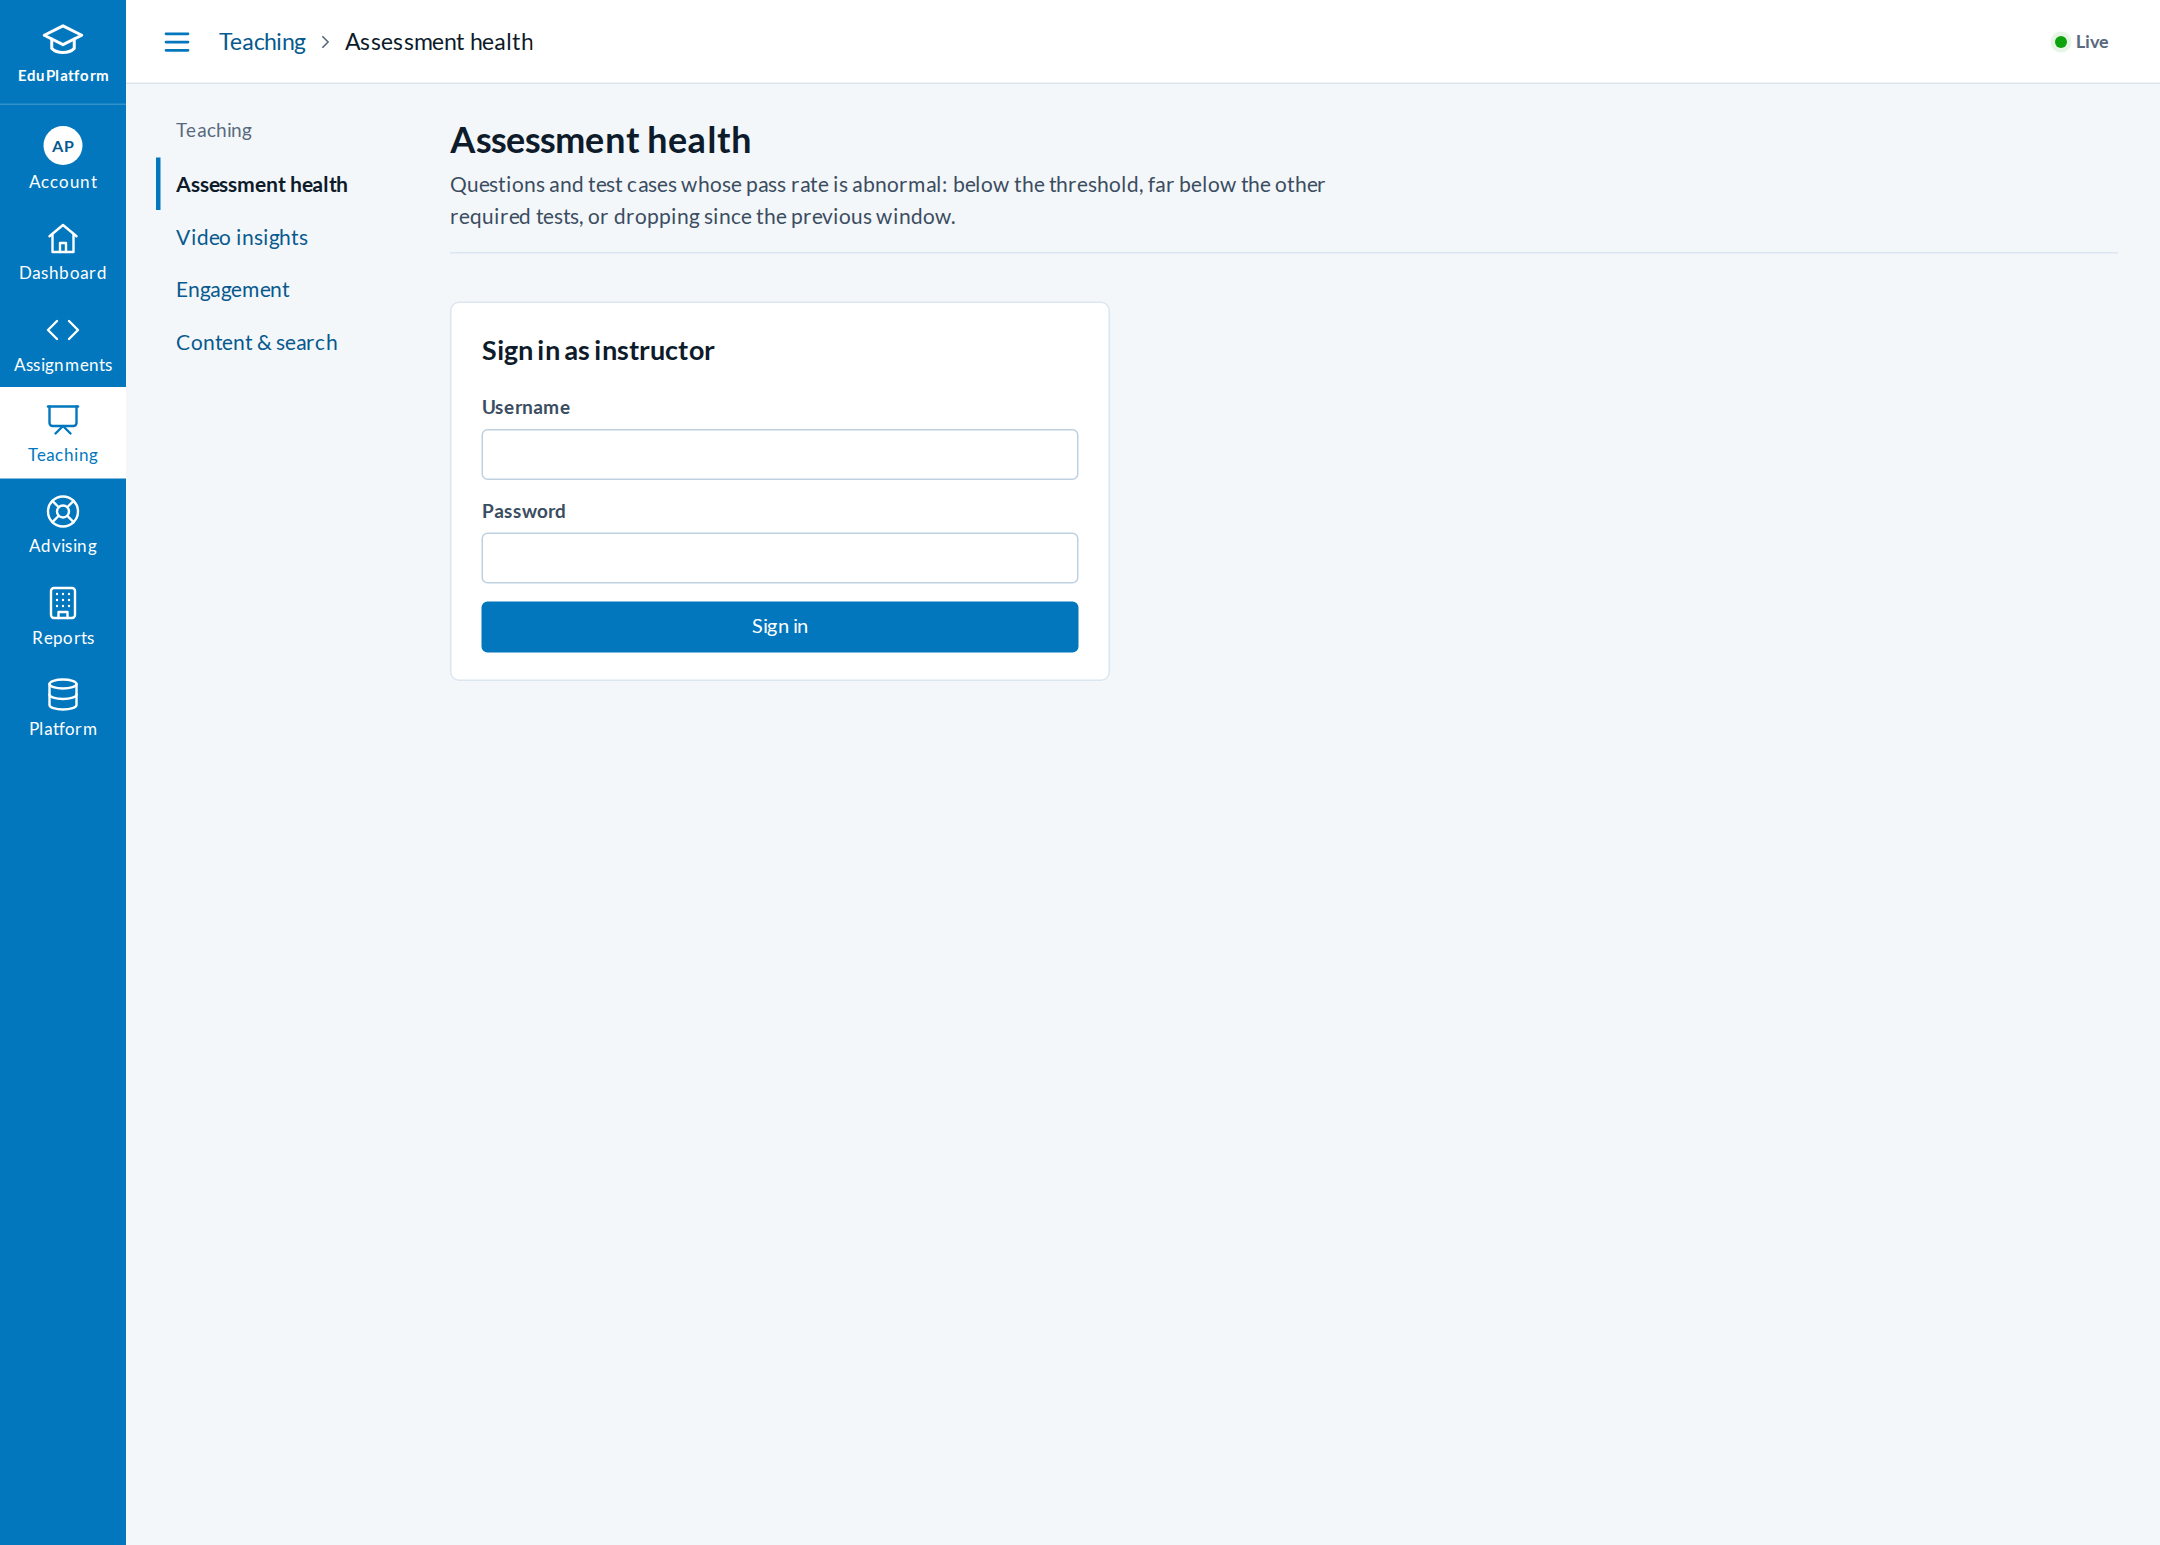
\includegraphics[width=\linewidth,trim=0 535bp 660bp 0,clip]{figures/current/auth-instructor.png}
  \caption{Instructor, Persistent}
\end{subfigure}\\[5pt]
\begin{subfigure}{0.48\textwidth}
  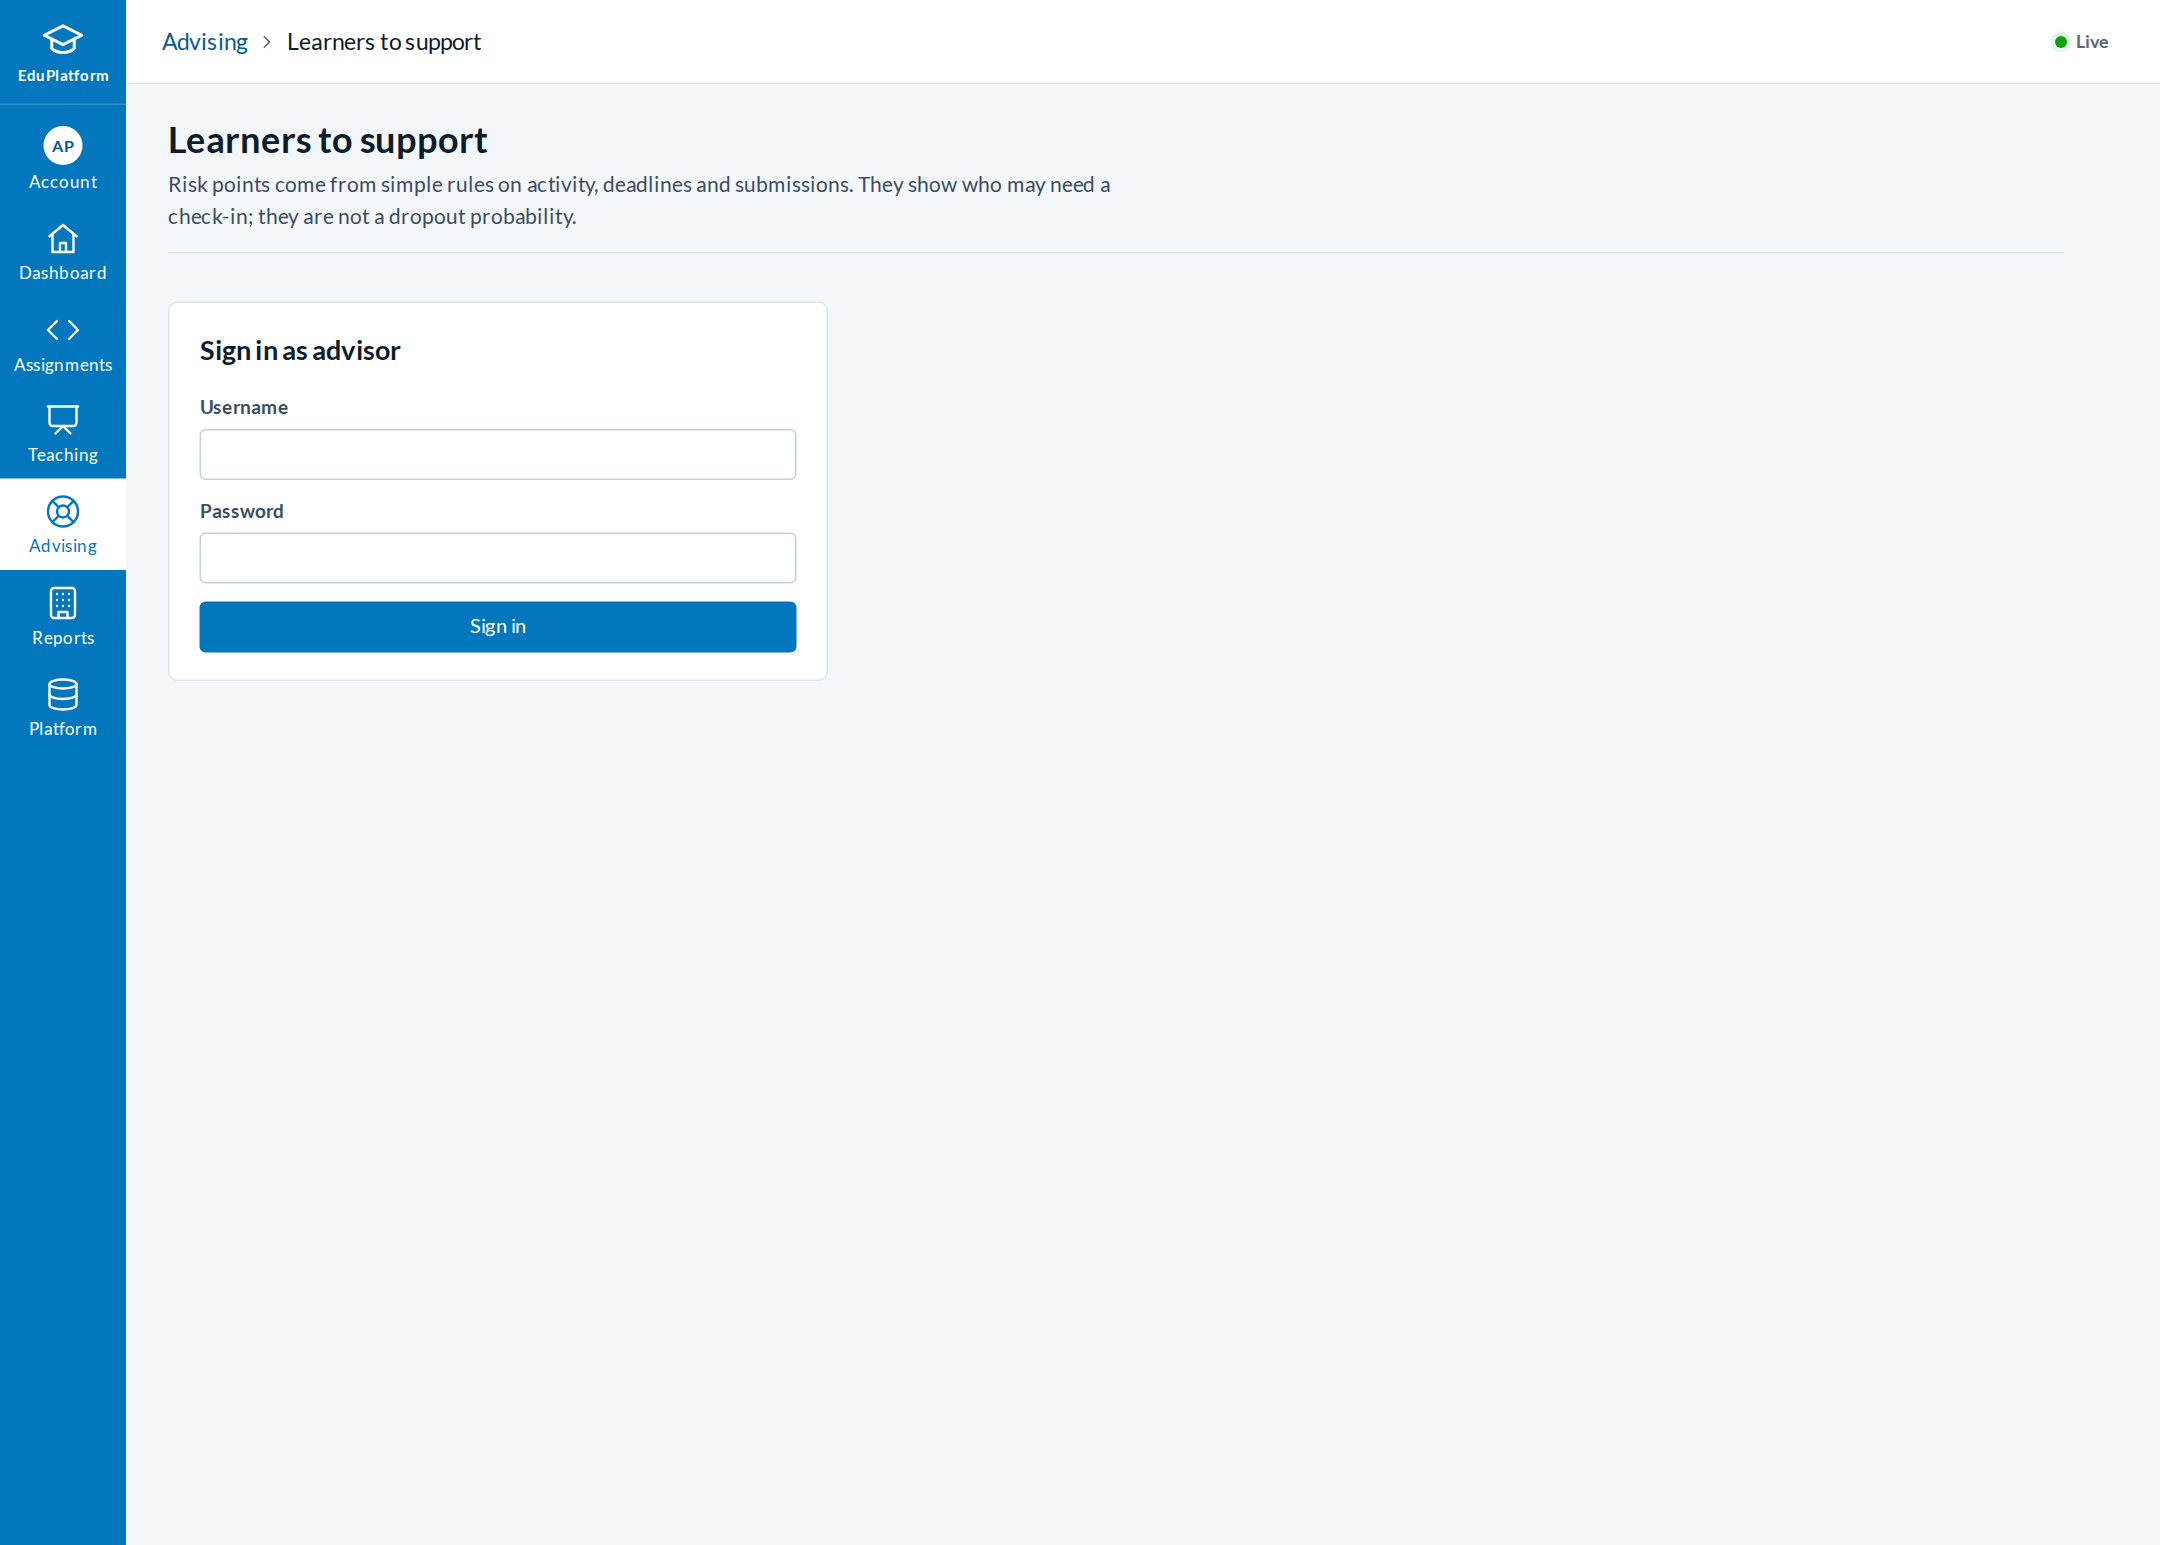
\includegraphics[width=\linewidth,trim=0 535bp 820bp 0,clip]{figures/current/auth-advisor.png}
  \caption{Advisor, Persistent}
\end{subfigure}\hfill
\begin{subfigure}{0.48\textwidth}
  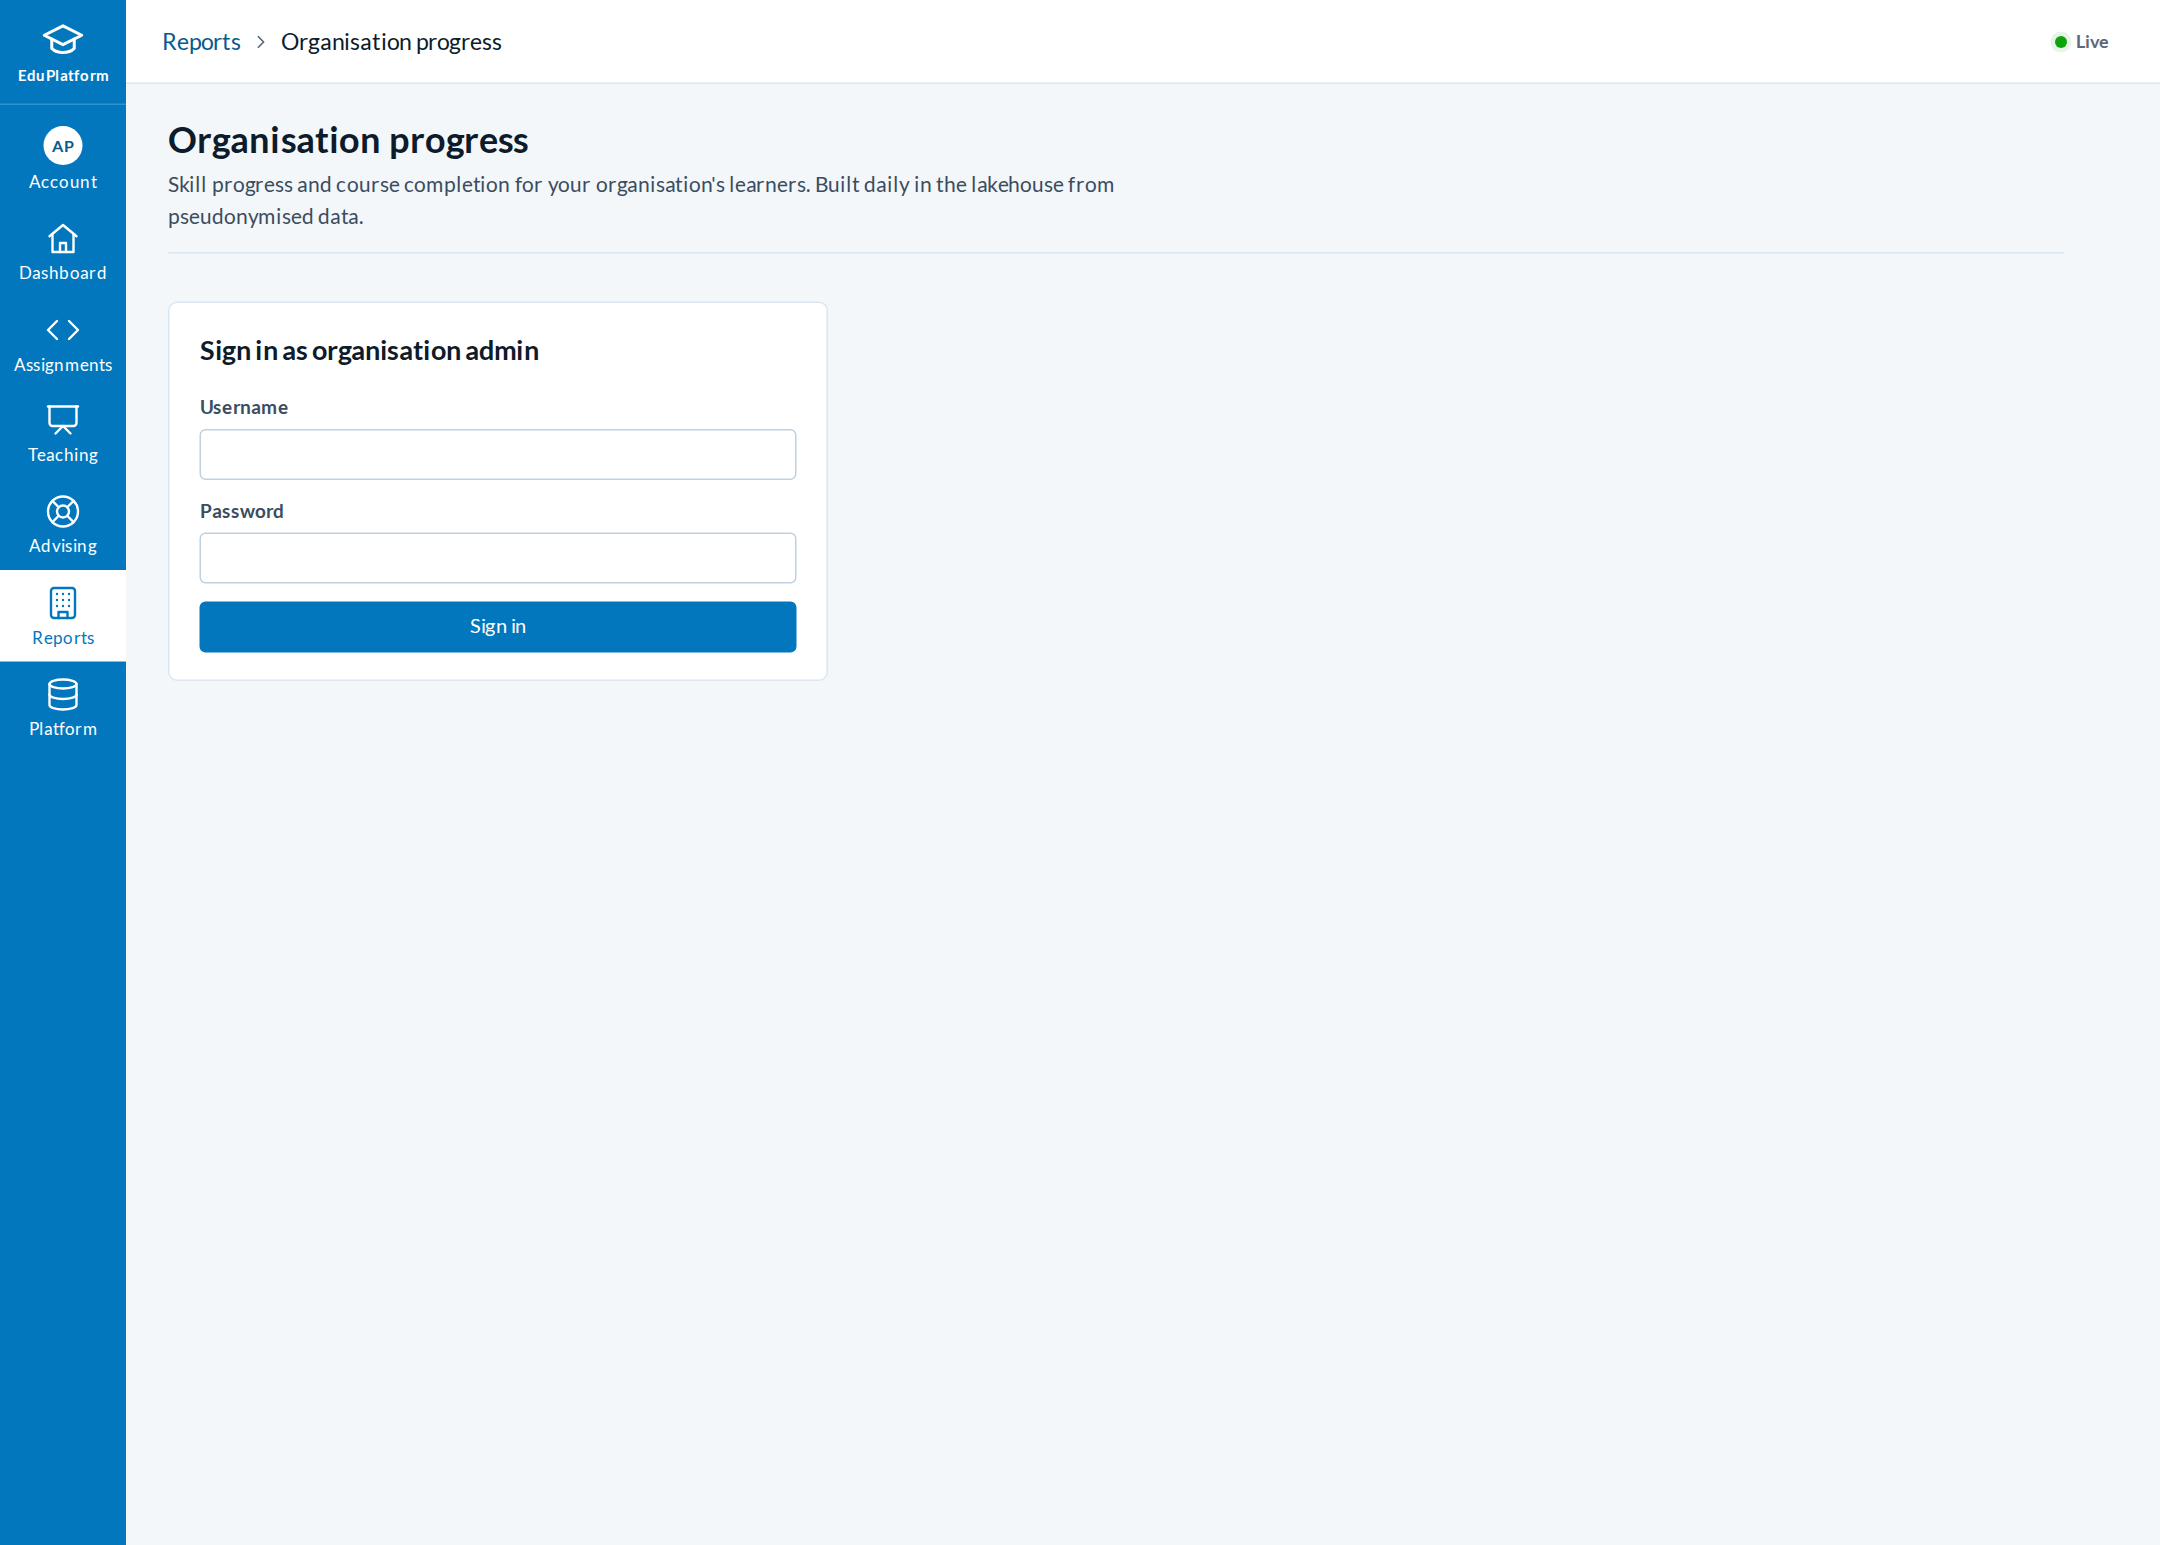
\includegraphics[width=\linewidth,trim=0 535bp 820bp 0,clip]{figures/current/auth-admin.png}
  \caption{Organisation Admin, Persistent}
\end{subfigure}
\caption{Form đăng nhập theo vai trò trước khi nhập mật khẩu}
\label{fig:ui-auth}
\end{figure}

\subsubsection{Các màn hình chính}

Các fixture là dữ liệu tổng hợp. Classroom lưu bài học và bài nộp vào PostgreSQL. Ảnh Persistent BR4/BR5 chụp sau khi kết quả đã đi qua CDC và worker chạy thật. Ảnh BR6--BR8 dùng các mart Trino và dịch vụ nội dung của stack báo cáo. Pipeline Health hiển thị luồng sự kiện demo của ứng dụng.

Giảng viên xem thay đổi sau sửa điểm ở Hình~\ref{fig:ui-br4} và~\ref{fig:ui-br4-corrected}. Cố vấn theo dõi cùng cảnh báo khi người học phục hồi ở Hình~\ref{fig:ui-br5} và~\ref{fig:ui-br5-recovered}. Quản trị viên xem ngưỡng công bố ở Hình~\ref{fig:ui-br6} và~\ref{fig:ui-br6-globex}, còn phạm vi phiên Acme được minh họa ở Hình~\ref{fig:ui-admin-scope}.

\newcommand{\currentui}[3]{%
  \begin{figure}[htbp]
  \centering
  \includegraphics[width=\textwidth,height=0.49\textheight,keepaspectratio]{figures/current/#1.png}
  \caption{#2}\label{#3}
  \end{figure}%
}

\newcommand{\uistate}[3]{%
  \begin{subfigure}{\textwidth}
  \centering
  \includegraphics[width=\linewidth,height=0.40\textheight,keepaspectratio]{figures/current/#1.png}
  \caption{#2}\label{#3}
  \end{subfigure}%
}

\currentui{learner-home}{Learner Home trong Classroom. Người học Chi thấy khoá học, thông báo và tiến độ bài học}{fig:ui-learner}
\currentui{code-lab}{Code Lab trong Classroom. Lời giải FizzBuzz nhận phản hồi đã chấm và kết quả theo test}{fig:ui-codelab}

\begin{figure}[p]
\centering
\uistate{assessment-health}{Trạng thái cơ sở có 2/24 lượt đạt và một test cần xem xét. Delta version 16}{fig:ui-br4}
\par\medskip
\uistate{assessment-corrected}{Sau sửa điểm qua CDC, worker Spark/Delta công bố 3/24 lượt đạt. Delta version 17}{fig:ui-br4-corrected}
\caption{Assessment Health trong Persistent với fixture Python for Data}
\end{figure}

\begin{figure}[p]
\centering
\uistate{advisor}{Học viên mẫu có 100 điểm và một cảnh báo mới}{fig:ui-br5}
\par\medskip
\uistate{advisor-recovered}{Sau bốn hoạt động mới, điểm giảm còn 50 và cảnh báo được giải quyết}{fig:ui-br5-recovered}
\caption{Vòng đời cảnh báo trong Learners to support, chế độ Persistent}
\end{figure}

\currentui{replay}{Assessment Health trong Replay, có nhãn Simulated data}{fig:ui-replay}
\currentui{video-insights}{Video Insights trong Persistent. Mart Trino hiển thị phiên bản 2 của video Joins đến 17/10/2026}{fig:ui-br7}
\currentui{engagement}{Engagement trong Persistent. Mart Trino hiển thị xu hướng theo tuần của SQL Foundations}{fig:ui-engagement}
\currentui{content-search}{Content \& Search trong Persistent. Transcript Joins đã đồng bộ và có thể tìm kiếm}{fig:ui-br8}
\begin{figure}[p]
\centering
\uistate{admin-acme}{Acme hiển thị số liệu của nhóm đủ điều kiện}{fig:ui-br6}
\par\medskip
\uistate{admin-globex}{Globex ẩn tỷ lệ và số hoàn thành của nhóm dưới 5 học viên}{fig:ui-br6-globex}
\caption{Organisation Progress trong Persistent với snapshot kho ngày 17/10/2026}
\end{figure}

\currentui{admin-scoped}{Phiên Admin chỉ có phạm vi Acme. Yêu cầu kiểm chứng đến API Globex trả 403}{fig:ui-admin-scope}
\currentui{pipeline}{Pipeline Health. Các bộ đếm và topic của luồng demo}{fig:ui-pipeline}

\begin{figure}[htbp]
\centering
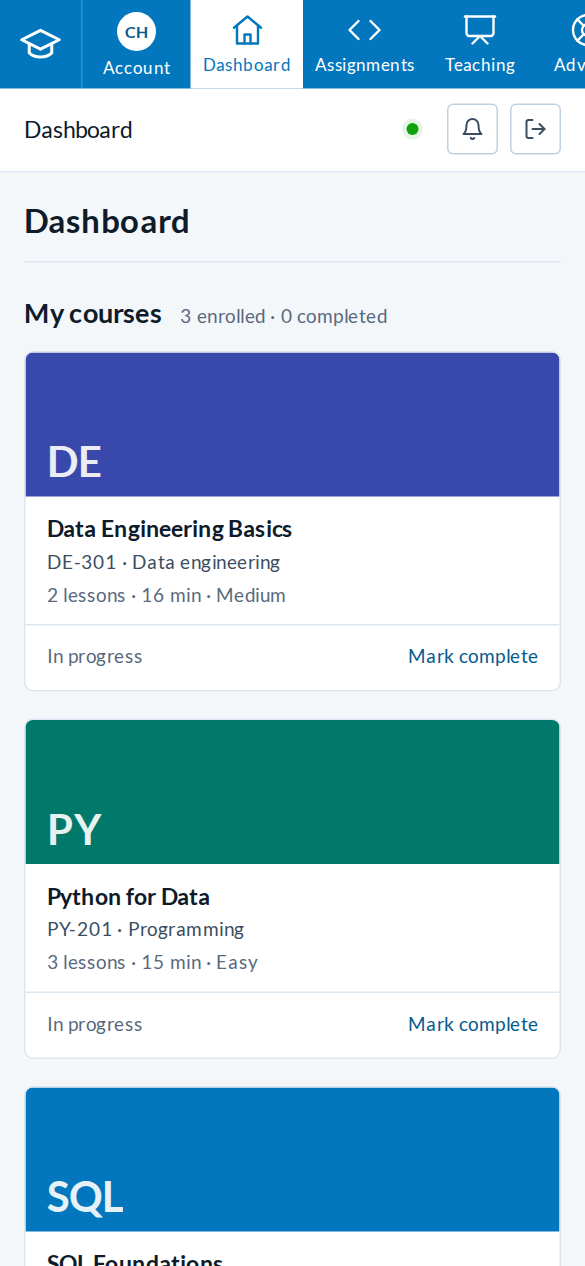
\includegraphics[width=0.35\textwidth,height=0.60\textheight,keepaspectratio]{figures/current/learner-mobile.png}
\caption{Learner Home trong Classroom ở chiều rộng 390 px}
\label{fig:ui-mobile}
\end{figure}

\subsubsection{Kiểm thử giao diện}

TypeScript ở chế độ nghiêm ngặt và bản build production đã qua kiểm tra. Năm lượt Playwright sau thay đổi auth kiểm tra phiên staff trong ba chế độ, Replay dùng chung kịch bản và bài nộp Code Lab trong Classroom. Các phép kiểm thử API xác nhận hết hạn, đăng xuất độc lập, kiểm tra quyền sở hữu Student, phạm vi staff và tương thích Bearer. Ảnh BR4/BR5 bổ sung minh chứng cho những thay đổi xuất hiện trên dashboard sau CDC. Bảng ánh xạ ảnh cũ, nguồn chụp và trạng thái được lưu cùng nguồn LaTeX.
